\documentclass[10pt,a4paper]{article}
\usepackage[utf8]{inputenc}
\usepackage[portuguese]{babel}
\usepackage[T1]{fontenc}
\usepackage{amsmath}
\usepackage{amsfonts}
\usepackage{amssymb}
\usepackage{graphicx}
\usepackage[left=2.5cm,right=2.5cm,top=2.5cm,bottom=2.5cm]{geometry}
\usepackage{listings}
\usepackage{color} %red, green, blue, yellow, cyan, magenta, black, white
\definecolor{mygreen}{RGB}{28,172,0} % color values Red, Green, Blue
\definecolor{mylilas}{RGB}{170,55,241}

\author{Murilo Camargos}
\title{Métodos Computacionais - Lista 1}
\begin{document}
\lstset{extendedchars=true, inputencoding=latin1,literate=
{á}{{\'a}}1
{à}{{\`a}}1
{ã}{{\~a}}1
{é}{{\'e}}1
{ê}{{\^e}}1
{í}{{\'i}}1
{ó}{{\'o}}1
{õ}{{\~o}}1
{ú}{{\'u}}1
{ü}{{\"u}}1
{ç}{{\c{c}}}1}
\lstset{language=Matlab,%
    %basicstyle=\color{red},
    breaklines=true,%
    morekeywords={matlab2tikz},
    keywordstyle=\color{blue},%
    morekeywords=[2]{1}, keywordstyle=[2]{\color{black}},
    identifierstyle=\color{black},%
    stringstyle=\color{mylilas},
    commentstyle=\color{mygreen},%
    showstringspaces=false,%without this there will be a symbol in the places where there is a space
    numbers=left,%
    numberstyle={\tiny \color{black}},% size of the numbers
    numbersep=9pt, % this defines how far the numbers are from the text
    emph=[1]{for,end,break},emphstyle=[1]\color{red}, %some words to emphasise
    %emph=[2]{word1,word2}, emphstyle=[2]{style},
    extendedchars=true,
    inputencoding=latin1, 
}


	\section{Método de Chebyshev (15/11/2017)}
	Seja $f(x)$ uma função limitada no intervalo $(a,b)$. Podemos expandir $f(x)$ da seguinte maneira:
	\begin{equation}
		f(x(t))_{(a\leq x\leq b)} = F(t) = \frac{1}{2}a_0 + a_1T_1(t) + a_2T_2(t) + \dots
		\label{eq:1}
	\end{equation}
	em que
	\[T_r(t) = \cos{\left(r \cos^{-1}{(t)}\right)}\]
	\[t = \frac{2x - (b+a)}{b-a}\]
	Integrando a Eq. \ref{eq:1}, temos:
	\begin{equation}
		\frac{2}{b-a}\int_a^xf(x)dx = \int_{-1}^tF(t)dt = \frac{1}{2}b_0+b_1T_1(t)+b_2T_2(t)+\dots
		\label{eq:2}
	\end{equation}
	em que
	\[b_r = \frac{a_{r-1}-a_{r+1}}{2r}, \hspace{1cm} r=1,2,3,\dots\]
	
	O valor de $b_0$ é determinado pelo limite inferior de integração, então:
	\[b_0 = 2b_1 - 2b_2 + 2b_3 - 2b_4 + \dots\]
	
	A integral é definida por:
	\begin{equation}
		\frac{2}{b-a}\int_a^bf(x)dx = \int_{-1}^1F(t)dt = \frac{1}{2}b_0+b_1+b_2+\dots = 2\left(b_1+b_3+b_5+\dots\right)
		\label{eq:3}
	\end{equation}
	
	Os coeficientes da expansão \ref{eq:1} podem ser calculados usando a observação de que qualquer polinômio de grau $N$ pode ser escrito na forma
	\begin{equation}
		f(x(t)) = F(t) = \frac{1}{2}a_0+a_1T_1(t)+a_2T_2(t)+\dots+a_{N-1}T_{N-1}(t)+\frac{1}{2}a_NT_N(t) = {\sum_{r=0}^N}'' a_rT_r(t)
		\label{eq:4}
	\end{equation}
	
	Aqui, ${\sum}''$ denota a soma finita sujo primeiro e último termos são multiplicados por $\frac{1}{2}$.
	
	Os coeficientes em \ref{eq:4} são dados por
	\[a_r = \frac{2}{N}{\sum_{s=0}^N}'' F\left(\cos{\frac{\pi s}{N}}\right)\cos{\left(\frac{\pi r s}{N}\right)}\]
	
	Isto é uma consequência da ortogonalidade da função cosseno com respeito aos pontos $t_s=\cos{\frac{\pi s}{N}}$, expressada pela equação:
	\[{\sum_{s=0}^N}'' \cos{\left(\frac{\pi i s}{N}\right)}\cos{\left(\frac{\pi j s}{N}\right)} = \begin{cases}0,&i\neq j\\N,&i=j=0\mbox{ ou }N\\\frac{1}{2}N,&i=j\neq 0\mbox{ ou }N\end{cases}\]
	
	\section{Exercícios (16/11/2017)}
	Use o método de expansão de Chebyshev para calcular as integrais definidas abaixo com até 6 dígitos de precisão. As integrais são:
	\[\int_{-1}^1 \frac{1}{x^2+x^2+0.9}dx\]
	\[\int_{-1}^1 \sqrt{\left|x+\frac{1}{2}\right|}dx\]
	\noindent Para cada caso, construa uma tabela de valores para os coeficientes $a_r$ e $b_r$. Obtenha, também, um gráfico da função aproximada pelo método e compare com o gráfico da função no integrando.
	
	\section{Resolução}
	
	O método de Chebyshev para cálculo de integrais definidas foi implementado em MATLAB
	
	\subsection{Exercício 1}
	Os valores de $a_r$ e $b_r$ são dados na tabela abaixo com $N=22$. Temos a seguinte integral definida:
    
    \[\int_{-1}^1 \frac{1}{x^4+x^2+0.9} dx.\]

    
    \begin{table}[h]
    \centering
    \caption{Resultados numéricos do primeiro exercício.}
    \label{my-label}
    \begin{tabular}{lrr}
\hline
 r   &   $a_r$               & $b_r$\\
 \hline
 0   &   1.336666674225290   &   -  \\
 1   &   0.000000000000000   &   0.858441127690537  \\
 2   &  -0.380215581155785   &   0.000000000000000  \\
 3   &  -0.000000000000000   &  -0.073545576067158  \\
 4   &   0.061057875247165   &  -0.000000000000000  \\
 5   &   0.000000000000000   &   0.006451618504673  \\
 6   &  -0.003458309799560   &   0.000000000000000  \\
 7   &   0.000000000000000   &  -0.000152793299825  \\
 8   &  -0.001319203602016   &  -0.000000000000000  \\
 9   &   0.000000000000000   &  -0.000102300550229  \\
10   &   0.000522206302106   &   0.000000000000000  \\
11   &  -0.000000000000001   &   0.000028448694199  \\
12   &  -0.000103664970276   &  -0.000000000000000  \\
13   &   0.000000000000000   &  -0.000004394783399  \\
14   &   0.000010599398091   &   0.000000000000000  \\
15   &  -0.000000000000000   &   0.000000325208060  \\
16   &   0.000000843156299   &   0.000000000000000  \\
17   &  -0.000000000000001   &   0.000000044054481  \\
18   &  -0.000000654696062   &  -0.000000000000000  \\
19   &   0.000000000000000   &  -0.000000021484507  \\
20   &   0.000000161715189   &  -0.000000000000000  \\
21   &   0.000000000000001   &   0.000000004921833  \\
22   &  -0.000000045001792   &   -  \\
\hline
    \end{tabular}
    \end{table}
    
    O valor da integral é dado por:
    	\[\int_{-1}^1 \frac{1}{x^4+x^2+0.9} dx = 2\left(b_1+b_3+b_5+\dots\right)=1.582232965777331\]
        
       Na aproximação da função do integrando, a raiz quadrada do erro quadrático médio foi de:
       \[\mbox{RMSE} = \sqrt{\frac{\sum_{i=1}^n\left(\hat{y}_t-y_t\right)^2}{n}} = 1.902886989865449\cdot 10^{-7}\]
    
    
    \begin{figure}
    	\centering
      \includegraphics[width=0.8\linewidth]{figures/f1.eps}
      \caption{Convergência dos valores de $b_r$ no exercício 1.}
      \label{fig:f1br}
	\end{figure}
    
    \begin{figure}
    \centering
      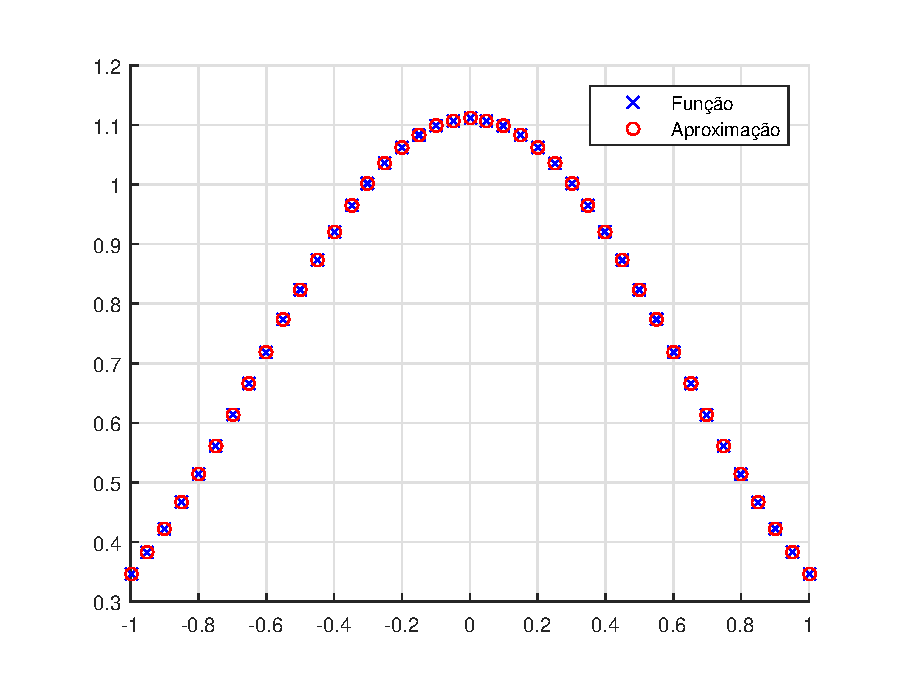
\includegraphics[width=0.8\linewidth]{figures/ap1.eps}
      \caption{Função do exercício 1 aproximada.}
      \label{fig:ap1br}
	\end{figure}
    
    \newpage
    \subsection{Exercício 2}
    
    Os valores de $a_r$ e $b_r$ são dados na tabela abaixo com $N=19$. Temos a seguinte integral definida:
    
    \[\int_{-1}^1 \sqrt{\left|x+\frac{1}{2}\right|} dx.\]
   
    
    \begin{table}[h]
    \centering
    \caption{Resultados numéricos do segundo exercício.}
    \label{my-label}
    \begin{tabular}{lrr}
\hline
 r   &   $a_r$               & $b_r$\\
 \hline
 0   &   1.579218322193437   &   -  \\
 1   &   0.366965847474833   &   0.706798543267637  \\
 2   &   0.165621235658162   &   0.127971400146460  \\
 3   &  -0.144919753111006   &   0.020615630793443  \\
 4   &   0.041927450897503   &  -0.022306267769967  \\
 5   &   0.033530389048728   &   0.008925014411228  \\
 6   &  -0.047322693214777   &   0.001260725493651  \\
 7   &   0.018401683124920   &  -0.004380237292847  \\
 8   &   0.014000628885079   &   0.002631724712030  \\
 9   &  -0.023705912267560   &   0.000161211385072  \\
10   &   0.011098823953786   &  -0.001510158617662  \\
11   &   0.006497260085674   &   0.001124821018122  \\
12   &  -0.013647238444891   &  -0.000062835382376  \\
13   &   0.008005309262690   &  -0.000610000383275  \\
14   &   0.002212771520264   &   0.000572724555622  \\
15   &  -0.008030978294732   &  -0.000147278518457  \\
16   &   0.006631127073971   &  -0.000218432570725  \\
17   &  -0.001041136031548   &   0.000318722594433  \\
18   &  -0.004205441136746   &  -0.000202050212572  \\
19   &   0.006232671621041   &  -  \\
\hline
    \end{tabular}
    \end{table}
    
    O valor da integral é dado por:
    	\[\int_{-1}^1 \sqrt{\left|x+\frac{1}{2}\right|} dx = 2\left(b_1+b_3+b_5+\dots\right)=1.465612854550713\]
        
        Na aproximação da função do integrando, a raiz quadrada do erro quadrático médio foi de:
       \[\mbox{RMSE} = \sqrt{\frac{\sum_{i=1}^n\left(\hat{y}_t-y_t\right)^2}{n}} = 0.033624284161012\]
    
    \begin{figure}
    \centering
      \includegraphics[width=0.8\linewidth]{figures/f2.eps}
      \caption{Convergência dos valores de $b_r$ no exercício 2.}
      \label{fig:f2br}
	\end{figure}
    
    \begin{figure}
    \centering
      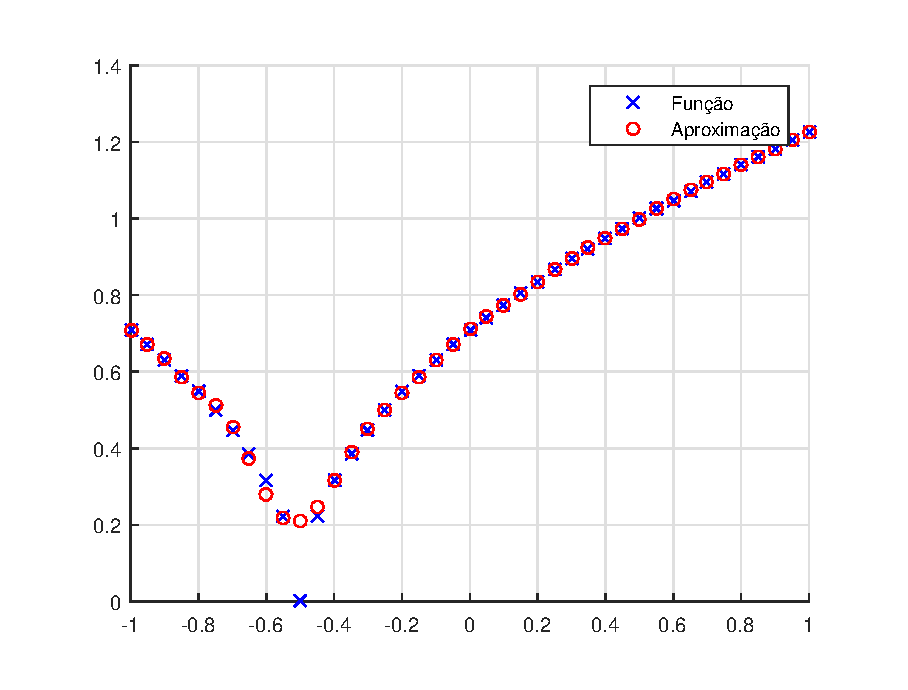
\includegraphics[width=0.8\linewidth]{figures/ap2.eps}
      \caption{Função do exercício 2 aproximada.}
      \label{fig:ap2br}
	\end{figure}
    
    \newpage
    \subsection{Código em MATLAB}
    \lstinputlisting{code/main.m}
    \subsection{Função de Chebyshev}
    \lstinputlisting{../tools/chebyshev.m}
    
\end{document}